% =====================================================================
%  MATH3030 Project Report
%  Build:  latexmk          (uses .latexmkrc -> XeLaTeX + biber)
% =====================================================================
\documentclass[a4paper, 11pt]{article}

% --- 1. Packages that do things (maths, figures, refs) ---------------
% =====================================================================
%  preamble.tex - functional packages only.
%  Nothing here should change how the document *looks*; that belongs in
%  themes/. Keep this file the same when you switch themes.
% =====================================================================

% --- Maths ------------------------------------------------------------
\usepackage{amsmath, amssymb, amsthm}
\usepackage{mathtools}

% --- Figures & tables -------------------------------------------------
\usepackage{graphicx}
\graphicspath{{figures/}}
\usepackage{subcaption}   % side-by-side figures: \begin{subfigure}
\usepackage{booktabs}     % nice tables: \toprule \midrule \bottomrule
\usepackage{float}
\usepackage{comment}      % \begin{comment} ... \end{comment} to hide blocks

% --- Bibliography -----------------------------------------------------
\usepackage[style=authoryear, backend=biber, maxcitenames=2]{biblatex}
%  Use \textcite{turing1952} -> "Turing (1952)"
%      \parencite{turk1991}  -> "(Turk 1991)"

% --- Links & cross-references (load hyperref late, cleveref last) -----
\usepackage{hyperref}
\usepackage[capitalise, noabbrev]{cleveref}
%  Use \cref{eq:gray-scott} -> "Equation 1", \cref{fig:spots} -> "Figure 2"

% --- Equation numbering by section: (2.1), (2.2), ... ------------------
\numberwithin{equation}{section}

% --- Theorem-like environments ----------------------------------------
\theoremstyle{definition}
\newtheorem{definition}{Definition}[section]
\newtheorem{example}[definition]{Example}
\theoremstyle{plain}
\newtheorem{theorem}[definition]{Theorem}
\newtheorem{proposition}[definition]{Proposition}
\theoremstyle{remark}
\newtheorem*{remark}{Remark}

% --- Drafting helper: \todo{...} shows in red; disable before submitting
\usepackage{xcolor}
\newcommand{\todo}[1]{\textcolor{red}{[TODO: #1]}}
% \renewcommand{\todo}[1]{}   % <- uncomment to hide all TODOs


% --- 2. Notation shortcuts -------------------------------------------
% =====================================================================
%  macros.tex - notation shortcuts. Define a symbol once here so it is
%  consistent everywhere, and can be changed in one place.
% =====================================================================

\newcommand{\R}{\mathbb{R}}
\newcommand{\diff}{\mathop{}\!\mathrm{d}}          % upright d: \diff t
\newcommand{\pd}[2]{\frac{\partial #1}{\partial #2}} % \pd{u}{t}
\newcommand{\lap}{\nabla^2}                          % Laplacian
\newcommand{\Jac}{J}                                 % Jacobian matrix
\DeclareMathOperator{\tr}{tr}                        % trace
% \det already exists in LaTeX

% Gray-Scott parameters (change symbols here if you switch convention)
\newcommand{\GSF}{F}
\newcommand{\GSk}{k}
\newcommand{\Du}{D_u}
\newcommand{\Dv}{D_v}


% --- 3. THEME: everything about how the document LOOKS ----------------
%  To change the look, point this at a different file in themes/.
%    themes/basic.tex  - plain LaTeX defaults (current)
%    themes/serif.tex  - Georgia + tighter margins, like your project plan
% =====================================================================
%  themes/basic.tex - a plain, safe starting look.
%  A theme file controls ONLY appearance: page size/margins, fonts,
%  heading style, spacing, colours, header/footer.
%  To make a new theme: copy this file, edit it, and change the
%  \input{themes/...} line in main.tex.
% =====================================================================

% --- Page layout ------------------------------------------------------
\usepackage[margin=2.5cm]{geometry}

% --- Fonts ------------------------------------------------------------
%  Default Latin Modern (works with pdfLaTeX and XeLaTeX).

% --- Paragraphs: space between, no indent ------------------------------
\usepackage[skip=6pt plus 1pt]{parskip}

% --- Links: no coloured boxes ------------------------------------------
\hypersetup{
  colorlinks = true,
  linkcolor  = black,
  citecolor  = black,
  urlcolor   = blue!50!black,
}


% --- 4. Bibliography --------------------------------------------------
\addbibresource{references.bib}

% --- Title information -------------------------------------------------
\title{Reaction Diffusion Systems and Turing Patterns}
\author{Ragav Srinivasan}
\date{\today}

\begin{document}

\maketitle

\begin{abstract}
	Procedural generation algorithms such as Perlin Noise are widespread in the Games and Entertainment industry. These algorithms can produce pseudo-realistic visuals of landscapes and natural vegetaion. However, they cannot produce organized patterns. Reaction Diffusion systems have been studied widely ever since Turing's paper on chemical morphogenesis which showed pattern formation resembling those found in biology. In this paper, we give a description turing patterns and study the patterns arising from the Gray Scott Model. I have done a Numerical simulation of the Gray Scott using a method provided by J.E Pearson to reproduce these patterns. Although not complete, the report intends to show how patterns can be used in computer graphics. 
\end{abstract}

\section{Introduction}
\label{sec:introduction}

This report is an exploration of Pattern formation from Reaction Diffusion Systems. 

% Structure 
\
% Describe each section in their own line:
\Cref{sec:background} gives the necessary context and background on this report, this includes a brief overview of procedural generation by Perlin Noise and it's limitations, an introduction to reaction diffusion systems, a discussion on Turing Patterns, and finally we will focus on pattern formation arising from the Gray Scott Model.   

\Cref{original} is my original contribution towards this topic featuring my stability analysis of the Gray Scott Model, A Numerical Simulation implementing a method proposed by \parencite{pearson1993} and finally a construction of a parameter map inspired by \parencite{munafo2022pearson}.   

\Cref{sec:conclusion} summarizes the research in this report and proposes the planned extensions of this topic that were unable to be featured this report. 


\section{Background}
\label{sec:background}
\subsection{Procedural Generation}
\label{sec:procedural}

Procedural generation is a broad set of techniques in computer graphics that is used to create visuals, such as pseudo-realistic textures, terrains and surfaces on the fly. It eliminates the need for artists to manually prototype and create their own worlds. Instead, a deterministic function called \emph{noise} is used to produce the desired visuals, on the fly as the player explores. This makes it possible to build large, \emph{lifelike} landscapes with mountains, rivers and vegetation with little impact on memory \parencite{lagae2010}.

% Examples of Procedural Generation

Procedural generation is based on many algorithms. In this section we study one of the most widely used algorithms: \emph{Perlin noise}.


% TODO: cite a source for the Tron / MAGI / Academy Award facts (e.g. Perlin's NYU biography page).
Ken Perlin devised his noise function after working on the visual effects for Disney's 1982 film \emph{Tron} at Mathematical Applications Group, Inc.\ (MAGI), and published it in 1985 \parencite{perlin1985}. His technique was so pivotal to the industry that it earned him an Academy Award for Technical Achievement \parencite{nyuperlin}, and it is still widely used in modern-day films and video games \parencite{lagae2010}.

Although, Perlin Noise has widespread use in the industry, There are some limitations.
Textures created with Perlin noise are random and have no structure \parencite{lagae2010}. Although this approach is ideal for terrain generation, it cannot be used to generate patterns found in biology such as coral reefs, zebra stripes, giraffe spots, etc. For this we use a different technique found in Reaction Diffusion Systems.


\subsection{Reaction Diffusion Systems}
\label{sec:rd-systems}

% Segue to reaction-diffusion systems
This brings us to the heart of this report: \emph{reaction-diffusion systems}. These are nonlinear dynamical systems, originally from chemistry, and models changes in concentrations of several chemical substances as they react and diffuse over space and time \parencite{turing1952}.

% Diffusion Behaviour
\emph{Diffusion} refers to the behaviour of chemical substances \textit{spreading} from regions of high concentration to low concentration and as a result the substance is uniformly distributed across a medium \parencite{britannicadiffusion}. It turns out that mathematically modelling this behaviour leads to an interesting variety of pattern formation called Turing patterns, which will be the focus of \cref{sec:turing-patterns}.

% General Form of Reaction Diffusion System
The general form of a reaction-diffusion system is
\begin{equation} \label{eq:rd-general}
	\pd{\mathbf{q}}{t} = D \nabla^2 \mathbf{q} + R(\mathbf{q}),
\end{equation}

% Explain the point of a dimensionless equation
Above is a dimensionless equation wherein all the physical quantities are stripped and all the terms scaled \parencite{strogatz}. 


The equation is above is dimensionless which means the physical quantities are stripped. This reduces the equation to include only a few parameters $F$ and $k$ making analysis much easier. \parencite{strogatz}.


\subsection{Turing patterns}
\label{sec:turing-patterns}

In 1952, towards the end of Alan Turing's life, Turing publishes one of his most seminal contributions in the field of mathematical biology. In his 1952 paper titled ``The Chemical Basis of Morphogenesis'', Turing discovers a mechanism which describes the formation of some patterns found in nature \parencite{turing1952}. For instance, the patterns found in animal skin such as the stripes of a zebra, spots of a jaguar, the structure of our brains and the formation of coral reefs are considered to be Turing patterns \parencite{sheffieldturing}.

In the paper, Turing studies the development of an embryo and describes a system of signalling molecules called \emph{morphogens}. The reaction and diffusion shown by these morphogens can destabilise the system leading to an interesting case of pattern formation \parencite{turing1952}.

In the following section, we will be studying Turing patterns formed by a simple model called the Gray-Scott model .

\subsection{The Gray-Scott model}
\label{sec:gray-scott}

% Describes the problem
The setup for the Gray-Scott model supposes that we have a \emph{well-mixed tank} of chemical $U$. Then the concentration of $U$. We are interested in knowing the concentration of the chemical in space and time. For this, we define a vector function $u(x, t)$  that is currently unknown. We assume that chemical $U$ has the same concentration in the spatial domain except for a small patch in the center of the tank where chemical $V$ is introduced into the system. \\
\\
In chemistry, the relationship between $U$ and $V$ is defined as \textit{autocatalysis} where the resulting product is a reactant, as is the case with $V$ in the reaction shown below. The relationship is akin to that of \textit{prey and predator} models.

\begin{equation*}
	\underbrace{U + 2V \to 3V}_{\text{$V$ reacts with $U$ to make more of itself}}
	\qquad
	\underbrace{V \to P}_{\text{decay}}
\end{equation*}


The second rule suggests decay for $V$ by turning into an inert product $P$ which means that it becomes a non-reactive substance.


% General form of the Gray Scott Model
\begin{align*}
	\frac{\partial U}{\partial t} & = D_u \nabla^2 U - UV^2 + F(1 - U) \\
	\frac{\partial V}{\partial t} & = D_v \nabla^2 V + UV^2 - (F + k)V
\end{align*}
% Explaination of the terms 
\begin{itemize}
	\item $D_u$ and $D_v$ are the diffusivities of chemicals $U$ and $V$.
	\item $U$ and $V$ are the unknown functions representing the concentrations of the respective chemicals in space and time.
	\item $F$ is the feed rate of chemical $U$.
	\item $k$ is the decay rate for chemical $V$.
    \item $\nabla^2$ is the laplacian operator calculates the average concentration of neighbouring molecules. 
\end{itemize}



\section{Original Contribution}
\label{sec:original}

\subsection{Linear Stability Analysis of the Gray-Scott Model}
\label{sec:stability}

Steady states of a dynamical system are states after which point the system shows no change. We consider a small disturbance around a steady state and say the state is \textit{stable} if the disturbance dampens and the system loops back to its steady state. While an \textit{unstable} steady state is when the disturbance grows and thus the system never returns back to its steady state \parencite{teschl2012}. To give an analogy, \cref{fig:ball-analogy} compares a ball on a hilltop versus in a valley. Panel (a) is a stable state as the ball returns to its steady state after a small nudge. Panel (b) is an example of an unstable state, the ball never returns to a steady state after a small push and finally panel (c) shows a bistable state where the ball returns to a steady state but at a different point.

\begin{figure}[htbp]
	\centering
	\begin{tikzpicture}[scale=0.9, >=Stealth]
		% --- (a) Stable: ball in a valley
		\begin{scope}
			\draw[thick] (-1.6,1.3) .. controls (-0.6,-0.6) and (0.6,-0.6) .. (1.6,1.3);
			\fill[blue!60] (0,0.1) circle (0.22);
			\draw[gray, dashed] (0.72,0.42) circle (0.22);
			\draw[->, thick, red!70!black] (0.62,0.85) to[bend right=30] (0.22,0.45);
			\node at (0,-0.9) {(a) Stable};
		\end{scope}
		% --- (b) Unstable: ball on a hilltop
		\begin{scope}[xshift=4.2cm]
			\draw[thick] (-1.6,-0.4) .. controls (-0.6,1.5) and (0.6,1.5) .. (1.6,-0.4);
			\fill[blue!60] (0,1.24) circle (0.22);
			\draw[gray, dashed] (0.4,1.17) circle (0.22);
			\draw[->, thick, red!70!black] (0.65,1.45) to[bend left=30] (1.25,0.55);
			\node at (0,-0.9) {(b) Unstable};
		\end{scope}
		% --- (c) Bistable: two valleys, a big push crosses the hill
		\begin{scope}[xshift=8.6cm]
			\draw[thick] (-2.0,1.2) .. controls (-1.6,-0.5) and (-0.9,-0.5) .. (-0.6,0.3)
			.. controls (-0.3,1.0) and (0.3,1.0) .. (0.6,0.3)
			.. controls (0.9,-0.5) and (1.6,-0.5) .. (2.0,1.2);
			\fill[blue!60] (-1.26,0.03) circle (0.22);
			\draw[gray, dashed] (1.26,0.03) circle (0.22);
			\draw[->, thick, red!70!black] (-1.0,0.5) .. controls (-0.3,1.9) and (0.3,1.9) .. (1.0,0.5);
			\node at (0,-0.9) {(c) Bistable};
		\end{scope}
	\end{tikzpicture}
	\caption{An analogy for Stability Analysis of Steady States}
	\label{fig:ball-analogy}
\end{figure}

Nonlinear systems such as the Gray-Scott model are difficult to solve analytically. Therefore, I will be doing a stability analysis to find out the behaviour of the system near its steady states. To do this, we will first linearise the system by its Jacobian matrix and classify by its trace and determinant.


% Why this analysis for gray scott 
In this analysis I will show how diffusion can \emph{destabilise} a steady state and result in pattern formation. The analysis will be done twice, once by dropping the coefficients of diffusion $D_u$ and $D_v$ and then we will add them back to the system and check whether it destabilises the system.


\begin{equation}
	\label{eq:gs-stab}
	\begin{aligned}
		\pd{U}{t} & = \Du \lap U + \underbrace{-UV^2 + \GSF(1 - U)}_{f(U,V)},   \\
		\pd{V}{t} & = \Dv \lap V + \underbrace{UV^2 - (\GSF + \GSk)V}_{g(U,V)}.
	\end{aligned}
\end{equation}

% =====================================================================
\subsubsection*{Stability Analysis without Diffusion}

Setting $\Du = \Dv = 0$ in \cref{eq:gs-stab}, every point in space will behave in the same way. We define $\dot{U}$ and $\dot{V}$:
\begin{equation}
	\label{eq:gs-nodiff}
	\begin{aligned}
		\dot{U} & = f(U, V) = -UV^2 + F(1 - U), \\
		\dot{V} & = g(U, V) = UV^2 - (F + k)V.
	\end{aligned}
\end{equation}


A steady state is when $f = g = 0$. Setting $g = 0$ and factorizing by $V$ gives us $g = V(UV + (F + k)) = 0$. Here, we have two cases for $V$. If $V  = 0$, then $U = 1$ which is our \emph{trivial steady state}.
\\
Let's first classify stability of  the trivial steady state by the Jacobian of the system given by:

\begin{equation}
	\label{eq:gs-jacobian}
	J =
	\begin{pmatrix}
		\dfrac{\partial f}{\partial U} & \dfrac{\partial f}{\partial V} \\[8pt]
		\dfrac{\partial g}{\partial U} & \dfrac{\partial g}{\partial V}
	\end{pmatrix}
	=
	\begin{pmatrix}
		-V^2 - F & -2UV          \\
		V^2      & 2UV - (F + k)
	\end{pmatrix}.
\end{equation}


To classify the steady state, we first substituted the point into the above Jacobian. Then calculate, $p = tr J$ and $q = det J$. The state is considered to be stable if $p < 0$ and $q > 0$.
\begin{equation}
	\label{eq:gs-jacobian-trivial}
	J(1, 0) =
	\begin{pmatrix}
		-F & 0        \\
		0  & -(F + k)
	\end{pmatrix},
	\qquad p = -(2F + k), \qquad q = F(F + k), \qquad p^2 - 4q = k^2 .
\end{equation}
Since $F, k > 0$, we have $p < 0$, $q > 0$ and $p^2 - 4q \geq 0$, so the trivial state is a \emph{stable node for every} $F$ and $k$. This suggests that when a small concentration of chemical $V$  is added to the tank mixed by $U$, the $V$ dies out and the system is back to its original state.

Next, we consider the second case where $UV + (F + k) = 0 \rightarrow UV = (F + k)$. Substituting $UV = (F + k)$ in $f(U,V)$ gives the set of non-trivial steady states:

\begin{equation}
	\label{eq:gs-nontrivial}
	\begin{gathered}
		V = \frac{F(1 - U)}{F + k}, \qquad
		U^2 - U + c = 0 \quad \text{with } c = \frac{(F + k)^2}{F}, \\[4pt]
		U_\pm = \frac{1}{2}\left(1 \pm \sqrt{1 - \frac{4(F + k)^2}{F}}\right), \qquad
		V_\pm = \frac{F + k}{U_\pm}.
	\end{gathered}
\end{equation}
The steady states only exist under the following condition:
\begin{equation}
	\label{eq:saddle-node}
	F \ge 4(F + k)^2 \Rightarrow \GSk \leq \tfrac{1}{2}\sqrt{F} - F .
\end{equation}

(Not complete) Doing further analysis from here will show that the non-trivial steady is stable.  

\subsubsection*{Adding back diffusion}
Not complete. 


\subsection{Simulation of the Gray--Scott Model} 

In \textit{Complex Patterns in a Simple System}, \textcite{pearson1993} numerically simulated the Gray-Scott model and found a wide variety of patterns across the
$(F, k)$ parameter space, including Turing-type patterns such as hexagonal arrays of
spots. He integrated the equations using the forward Euler method on a
$256 \times 256$ grid and classified the resulting patterns into 14 classes. 

Because \textcite{pearson1993} simulated the system with an initial condition consisting of a small square in the center of the grid with $(U, V) = (\tfrac{1}{2}, \tfrac{1}{4})$, his simulation missed several types of pattern. This observation was made by Robert Munafo \parencite{munafo2022pearson}, who extended Pearson's simulations with other starting conditions and plotted a parameter map of $F, k$ values and showed that there are actually 19 classes of patterns in the Gray-Scott model.  

Inspired by the work of \textcite{pearson1993} and \textcite{munafo2022pearson}, I will be implementing my own simulation using Pearson's Method to produce some examples of these patterns. I will also build my own version of Munafo's parameter map to show which patterns the Gray-Scott model produces with which parameters.


% My implementation
I implemented the simulation in a Python Notebook using NumPy. The Laplacian is computed for the whole grid at once with a  five point stencil. The values for the diffusion
rates are $D_u = 0.2$ and $D_v = 0.1$ and a time step of 0.1. Following Pearson, each run starts from the square of
$(U, V) = (\tfrac{1}{2}, \tfrac{1}{4})$ at the centre of the grid with $1\%$ 


I implemented the simulation in a Python Notebook using Numpy and plotted the results with Matplotlib (Code is given in the appendix). The parameters for the simulation are $D_u = 0.2$ and $D_v = 0.1$ with a time step of $dt = 1$. The initial conditions in the simulation are the same as Pearson's where the concentrations of $U$ and $V$ in the center of the grid are 0.5 and 0.25 respectively. I then chose the parameter $F = 0.022, k = 0.051$ value from \parencite{munafo2022pearson}.    

\cref{fig:coral} shows the result of a stepwise simulation using parameters $F = 0.022, k = 0.051$. 

\begin{figure}[htbp]
	\centering
	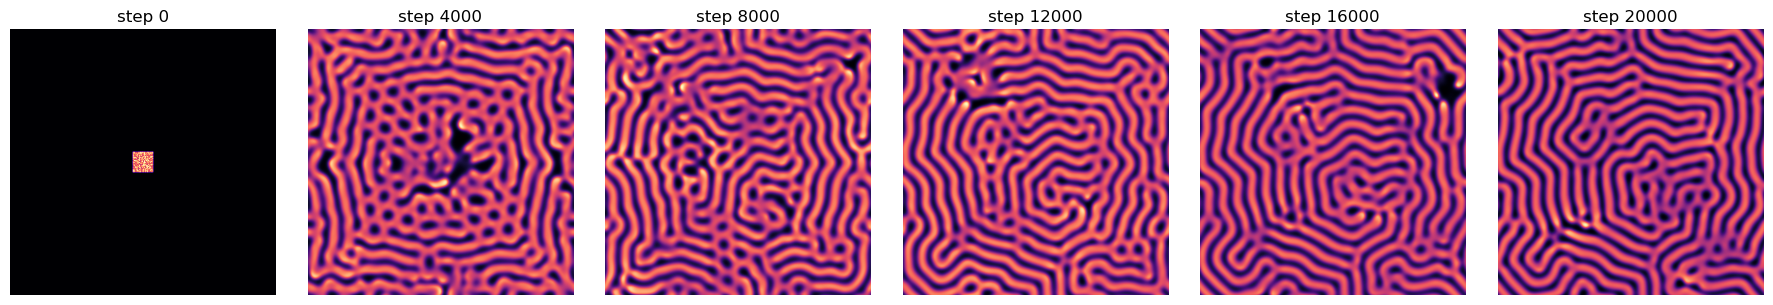
\includegraphics[width=\textwidth]{coral.png}
    \caption{Simulation of the Gray Scott model on $F = 0.022, k = 0.051$}  % write caption here
	\label{fig:coral}
\end{figure}
The results show a coral like reef like pattern. 

\subsection{Parameter Map}
Not complete


\section{Conclusion}
\label{sec:conclusion}
In conclusion, This report looked at a widely used technique in Computer Graphics called \emph{Perlin Noise} which is used to produce pseudo-realistic graphics of natural landscapes, vegetation and surfaces such as marble, wood, etc. Although a very useful algorithm, it's visuals are random and lack structure and is not the ideal algorithm to generate textures in biology. For this, we introduce Reaction Diffusion systems which is shown produce certain patterns that resemble biology, followed by a discussion of Alan Turing's 1952 paper on the "Chemical Basis of Morphogenesis" where he proposed a mechanism for pattern formation in biology by adding diffusion to a system modelling the development of an embryo. Finally, we studied the Gray-Scott model       


Due to time constraints, the report does not cover the intended goal of applying Reaction Diffusion systems to Computer Graphics. However, it is possible to use the results of from our numerical simulation in creating texture maps that can be used in 3D Design and Game development tools such as Blender, Godot, Unity and Unreal Engine. This will enable artists to produce graphics of natural phenomenon whose patterns can be explained by Reaction Diffusion. 

This report also attempts to do a stability Analysis on the Gray Scott Model with Diffusion. An analysis without the diffusion terms was done in this report which showed that the steady states of the model were stable. However, further analysis after adding back diffusion terms is still pending. I hypothesize that adding back diffusion to the system should destabilize the system as shown by \parencite{turing1952}, I believe this analysis could be helpful in identifying which parameters lead to stable and unstable states.   

Additionlly, a parameter map was also planned but the section stands incomplete due to falling short of time. 
\printbibliography

\pagebreak

\section{Project Plan}
\label{sec:plan}

\subsection*{Project plan as of 23rd October}

\subsubsection*{Project title}
Reaction Diffusion Systems and Turing Patterns

\subsubsection*{Overview}
This research paper will focus on the applications of Reaction Diffusion Systems. Reaction Diffusion systems emerge from Chemistry and Biology, however have found use in a lot of areas. The project will provide a background to Reaction Diffusion Systems, explore real world applications and document my own application for using it as a procedural generation algorithm (Python Program).

\subsubsection*{Required reading and sources}
To make it easier to start my research, I have structured my reading by effort: \emph{low effort}, \emph{medium effort} and \emph{high effort}.

\begin{enumerate}
  \item \emph{Low effort}: Short reading times of 15 to 30 minutes, aimed to give a basic understanding of the topic I'm researching. Videos from YouTube are also included in this category:
  \begin{itemize}
    \item \href{https://en.wikipedia.org/wiki/Reaction%E2%80%93diffusion_system}{Wikipedia: Reaction--diffusion system} and \href{https://en.wikipedia.org/wiki/Turing_pattern}{Turing pattern}: overview of the model and its biological motivation.
    \item \href{https://thecodingtrain.com/challenges/13-reaction-diffusion}{Coding Train: Coding Challenge \#13, Reaction Diffusion Algorithm} (\href{https://www.youtube.com/watch?v=BV9ny785UNc}{YouTube}): live implementation of the Gray--Scott model in p5.js.
    \item \href{https://karlsims.com/rd.html}{Karl Sims: Reaction-Diffusion Tutorial}: intuitive explanation of feed/kill rates, the discrete Laplacian, and the $(k, f)$ parameter map.
  \end{itemize}

  \item \emph{Medium effort}: Semi-long reading times of 30 to 45 minutes, aimed to give a more technical understanding of the topic with definitions and theorems related to the topic. Reading material includes longer videos, tutorials for math concepts from textbooks / internet, etc.
  \begin{itemize}
    \item \href{https://www.mrob.com/pub/comp/xmorphia/index.html}{Robert Munafo: Reaction-Diffusion by the Gray-Scott Model, Pearson's Parametrization}: term-by-term breakdown of the PDEs and a classified map of pattern types across parameter space.
    \item \href{https://redblobgames.com/x/2202-turing-patterns}{Red Blob Games: Turing Patterns notes}: worked exploration of Gray--Scott, including parameter sensitivity and convention differences between sources.
    \item \href{https://nbviewer.jupyter.org/github/numerical-mooc/numerical-mooc/blob/remove_pyc/lessons/04_spreadout/04_06_Reaction_Diffusion.ipynb}{Numerical MOOC: Reaction-Diffusion notebook}: forward-time/central-space discretisation of Gray--Scott in Python.
    \item Strogatz, \emph{Nonlinear Dynamics and Chaos} (2nd ed.), Ch.\ 5--6 (linear systems, phase plane) and Ch.\ 8 (bifurcations in 2D): the linearisation and trace--determinant tools needed for Turing stability analysis.
    \item \href{https://doi.org/10.1126/science.1179047}{Kondo \& Miura (2010), Reaction-diffusion model as a framework for understanding biological pattern formation}, \emph{Science}: accessible review connecting the theory to real animal patterns.
  \end{itemize}

  \item \emph{High effort}: Long reading times of up to 60 minutes. The reading material is much more complex and targeted, requires a lot of effort to understand. Material includes research papers, advanced math topics and full lectures:
  \begin{itemize}
    \item \href{https://doi.org/10.1098/rstb.1952.0012}{Turing (1952), The Chemical Basis of Morphogenesis}, \emph{Phil.\ Trans.\ R.\ Soc.\ B}: the original diffusion-driven instability argument.
    \item \href{https://arxiv.org/abs/patt-sol/9304003}{Pearson (1993), Complex Patterns in a Simple System}, \emph{Science} 261: the Gray--Scott parameter classification used by most graphics implementations.
    \item \href{https://doi.org/10.1145/122718.122749}{Turk (1991), Generating Textures on Arbitrary Surfaces Using Reaction-Diffusion}, SIGGRAPH '91: reaction-diffusion applied directly to 3D surfaces.
    \item \href{https://doi.org/10.1145/122718.122750}{Witkin \& Kass (1991), Reaction-Diffusion Textures}, SIGGRAPH '91: anisotropic and spatially varying reaction-diffusion for texture synthesis.
    \item Murray, \emph{Mathematical Biology II: Spatial Models and Biomedical Applications} (3rd ed.), Ch.\ 2: full derivation of the Turing instability conditions and the critical wavenumber, which is the core of the linear stability analysis.
  \end{itemize}
\end{enumerate}

\subsubsection*{What I'll do}
The research project will start with an introduction of the chosen research topic: \emph{Reaction Diffusion Systems} and \emph{Turing Patterns}. Then I plan to investigate the solutions of this family of equations and determine the behaviour. After this, I'm planning to highlight several applications of this topic that I've found from my research. In the end, I would like to wrap up this report with my original contribution of developing a program in Python that is capable of simulating and rendering patterns from Reaction Diffusion Systems.

\subsubsection*{Original contribution}
My original contribution to this report will include using the knowledge I've gained from this research topic and apply it to develop a Python program capable of producing Turing patterns.

\subsubsection*{Timeline}
Timeline as of 30th October:
\begin{itemize}
  \item[$\boxtimes$] Revised project plan, timeline and gather reading material
  \item[$\boxtimes$] Read material, take notes and make timeline more specific
  \item[$\boxtimes$] Read more material, take notes and write everything I've learned from my reading
  \item[$\boxtimes$] Define the right scope for the project and start thinking about ideas for original contribution
  \item[$\boxtimes$] 30th October: Research and take notes
  \item[$\square$] Focus on original contribution
  \item[$\square$] Finish original contribution by 1st November
  \item[$\square$] Send project for feedback
  \item[$\square$] Act on feedback and revise original contribution
  \item[$\square$] Complete introduction and conclusion sections by 5th November
  \item[$\square$] Send project for feedback before next week's class
  \item[$\square$] Proofread the project, look for issues
  \item[$\square$] Fix those issues
  \item[$\square$] 8th November: Project submission
\end{itemize}

\subsubsection*{Version control}
The research project is tracked using GitHub. The repository of the project can be accessed at: \url{https://github.com/Rageon787/math3030-project.git}

\subsubsection*{Plan revisions}
Revised plan with new timeline as I've fallen behind a lot. Future revisions will be about the scope of the project and original contribution.

\pagebreak
\section{Reflection}
When I first started working on this project, I had set myself some high expectations on this project. In the end, the plan I gave myself turned out to be unrealistic. I made revisions to the project each time I fell behind on progress. The final update to the project plan was on 23rd October as at the time I felt like I had a firm idea for my report. The checklists i made for myself didn't turn out to be realistic given my speed on this project and my workload from other units. 

I chose this topic because of my interest in Computer Graphics enjoy its use for mathematics and found Reaction Diffusion Systems to be link between nonlinear dynamics and computer graphics. In hindsight, I'm not sure if it turned out to be a good idea do something that interested as it created a lot of bias in the research.   

I planned the report to be a study on a specific Reaction Diffusion model called the Gray Scott Model. For the original contribution, I wanted to do a stability analysis and my own simulation of the Grey Scott Model using a method described by Pearson in his paper \textit{Complex Patterns in a Simple System} \parencite{pearson1993}. However, when i started doing the stability analysis for the Gray Scott Model with Diffusion I personally found it to be very difficult. So in my report, I’ve only been able to do a stability analysis of a single aspect of the model. 

I planned my report to be a study on Turing Patterns formed by Reaction Diffusion Systems. There is a fair amount of literature on the topic of Turing Patterns including Turing's discovery of these patterns in 1952, Pearson's numerical simulation \parencite{pearson1993} on the Gray Scott Model.   

I’m not very proud with the current state of my report as it stands incomplete and there are a lot of unanswered research questions. Although, I have stopped working on this report now. I find the topic fascinating so I've made the commitment to keep learning more about this topic in preparation for my viva exam and beyond. Specifically, I want to fill the gap in my stability analysis in which I couldn't complete further analysis of the non-trivial steady states and the part of adding back the diffusion coefficients. 

I deeply regret not asking for a lot of feedback on my project. I didn't feel confident send my report as I felt it wasn't coherent enough to read. I also spent a majority writing text for my report in a notebook as I felt it was much faster than typing. 


On a positive note, Doing this research project has given me a better grasp of Nonlinear Dynamics and the numerical methods for solving a system of Partial Differential Equations that I learned last semester. 


\section{Appendix}
\label{sec:appendix}
This appendix contains the Python code used for the simulation in \cref{sec:numerical}.

\subsection{Initial conditions}
\lstinputlisting{appendix_code/initial_state.py}

\subsection{Laplacian and forward Euler step}
\lstinputlisting{appendix_code/laplacian_and_euler.py}


\end{document}

